%% ============================================================
%%  MDLM Bug Fixer — Final Project Report
%%  Compile with: pdflatex report.tex  (or xelatex / lualatex)
%% ============================================================
\documentclass[11pt,a4paper]{article}

%% --- Packages ---
\usepackage[margin=1in]{geometry}
\usepackage{amsmath,amssymb}
\usepackage{graphicx}
\usepackage{booktabs}
\usepackage{multirow}
\usepackage{array}
\usepackage{xcolor}
\usepackage{hyperref}
\usepackage{listings}
\usepackage{subcaption}
\usepackage{float}
\usepackage{enumitem}
\usepackage{tikz}
\usetikzlibrary{shapes.geometric, arrows.meta, positioning, fit, calc, backgrounds}
\usepackage{pgfplots}
\pgfplotsset{compat=1.18}
\usepackage{microtype}
\usepackage{titlesec}
\usepackage{parskip}
\usepackage{caption}
\usepackage{algorithm}
\usepackage{algpseudocode}
\usepackage{mdframed}

%% --- Hyperref setup ---
\hypersetup{
    colorlinks=true,
    linkcolor=blue!70!black,
    citecolor=green!50!black,
    urlcolor=blue!70!black,
}

%% --- Listing style ---
\lstdefinestyle{python}{
    language=Python,
    basicstyle=\ttfamily\footnotesize,
    keywordstyle=\color{blue},
    commentstyle=\color{gray},
    stringstyle=\color{orange!80!black},
    breaklines=true,
    frame=single,
    numbers=left,
    numberstyle=\tiny\color{gray},
    xleftmargin=1.5em,
    framexleftmargin=1.2em,
}

%% --- TikZ styles (reused across diagrams) ---
\tikzset{
  block/.style={rectangle, rounded corners=4pt, draw=black!70, fill=blue!12,
                text width=5em, align=center, minimum height=2.2em, font=\footnotesize},
  wideblock/.style={block, text width=8em},
  bigblock/.style={block, text width=10em, minimum height=2.5em},
  arrow/.style={-Stealth, thick, draw=black!60},
  dasharrow/.style={-Stealth, thick, dashed, draw=gray!70},
  label/.style={font=\scriptsize\itshape, text=gray!70!black},
  groupbox/.style={draw=gray!50, dashed, rounded corners=6pt, inner sep=6pt},
}

%% --- Title ---
\title{%
  \textbf{Multi-Hunk Java Bug Repair via Masked Diffusion Language Models}\\[0.4em]
  \large A LoRA Fine-Tuned Iterative Denoising Approach with Baseline Comparisons
}
\author{Bhavya Gupta}
\date{March 2026}

%% ============================================================
\begin{document}
\maketitle
\tableofcontents
\newpage

%% ============================================================
\section{Abstract}
%% ============================================================

We present \textbf{MDLM Bug Fixer}, a system for automatically repairing Java programs that require simultaneous edits across \emph{multiple disjoint code regions} (hunks). Unlike autoregressive (AR) code models that generate patches sequentially, our approach leverages \textbf{LLaDA-8B-Instruct}~\cite{llada2024}—a Masked Diffusion Language Model (MDLM)—to fill all corrupted regions in parallel via iterative denoising.

We fine-tune LLaDA-8B with Low-Rank Adaptation (LoRA) on a preprocessed Java bug dataset derived from \texttt{bugs\_java.jsonl}, constructing \(2^k - k - 1\) training examples per file with \(k\) valid hunks. At inference, the model iteratively unmasks tokens in a confidence-ordered schedule. We compare against two zero-shot baseline families—FIM chaining (DeepSeek-Coder, StarCoder2, CodeLlama) and instruction-tuned zero-shot (Qwen2.5-Coder, DeepSeek-Instruct)—using a shared evaluation suite covering token exact match, patch BLEU, CodeBLEU, normalised edit distance, and pass@\(k\). Additionally, we evaluate on the Defects4J Java benchmark in an oracle-localised setting and on standard coding benchmarks (HumanEval, MBPP).

%% ============================================================
\section{Introduction}
%% ============================================================

Automated Program Repair (APR) aims to reduce the manual effort of debugging by automatically generating correct program patches from buggy code. A fundamental challenge in real-world APRs is that many patches require changes at \textbf{multiple, non-contiguous locations} within a single file—a scenario called \emph{multi-hunk repair}. Sequential autoregressive models handle multi-hunk repairs awkwardly: they must either generate all patches in a single forward pass or chain multiple FIM (Fill-In-the-Middle) passes with no global view of inter-hunk dependencies.

Masked Diffusion Language Models offer a natural fit for this task. By masking all hunk tokens simultaneously and denoising iteratively, the model can reason about inter-hunk consistency during every denoising step. Our key contributions are:

\begin{enumerate}[leftmargin=*, label=\textbf{\arabic*.}]
  \item A data preprocessing pipeline that identifies multi-hunk diffs from Java bug datasets, tokenises them with the LLaDA tokeniser, and constructs all valid hunk-subset training examples.
  \item A LoRA fine-tuning protocol for LLaDA-8B-Instruct targeted at multi-hunk infilling.
  \item A custom iterative denoising inference loop with confidence-based and random re-masking strategies.
  \item A systematic comparison against five FIM and instruct zero-shot baselines with a shared evaluation harness.
  \item Integration with the Defects4J benchmark suite for end-to-end oracle-localised Java bug repair evaluation.
\end{enumerate}

%% ============================================================
\section{Related Work}
%% ============================================================

\paragraph{Autoregressive models for code repair.}
Large code models such as CodeLlama~\cite{codellama}, StarCoder2~\cite{starcoder2}, DeepSeek-Coder~\cite{deepseek}, and Qwen2.5-Coder support fill-in-the-middle (FIM) pre-training that enables single-hunk infilling. Multi-hunk extension requires sequential chaining, where each filled hunk updates the context for the next—a strategy evaluated as our primary baseline.

\paragraph{Diffusion models for language.}
Masked language models such as BERT~\cite{bert} showed the power of non-autoregressive infilling. Masked Diffusion Language Models (MDLMs) formalise this as a continuous-time Markov chain over discrete tokens~\cite{austin2021structured, sahoo2024mdlm}. LLaDA~\cite{llada2024} scales this to 8B parameters with instruction tuning, using a learned \texttt{<|mdm\_mask|>} token as the diffusion noise state.

\paragraph{Automated program repair.}
APR benchmarks include Defects4J~\cite{defects4j} (Java), SWE-bench~\cite{swebench} (Python), and HumanEval~\cite{humaneval}. Prior work includes template-based repairs~\cite{genprog}, learning-based approaches~\cite{drrepair}, and LLM-based systems~\cite{chatrepair}. Most focus on single-hunk repairs; multi-hunk remains an open challenge.

%% ============================================================
\section{System Architecture}
%% ============================================================

\subsection{Overview}
\label{sec:arch}

Figure~\ref{fig:arch} provides a high-level view of the end-to-end system. It consists of four main stages: (1)~data preprocessing, (2)~LoRA fine-tuning, (3)~iterative denoising inference, and (4)~evaluation and benchmarking.

%% -----------------------------------------------
%%  ARCHITECTURE DIAGRAM — TikZ
%% -----------------------------------------------
\begin{figure}[H]
\centering
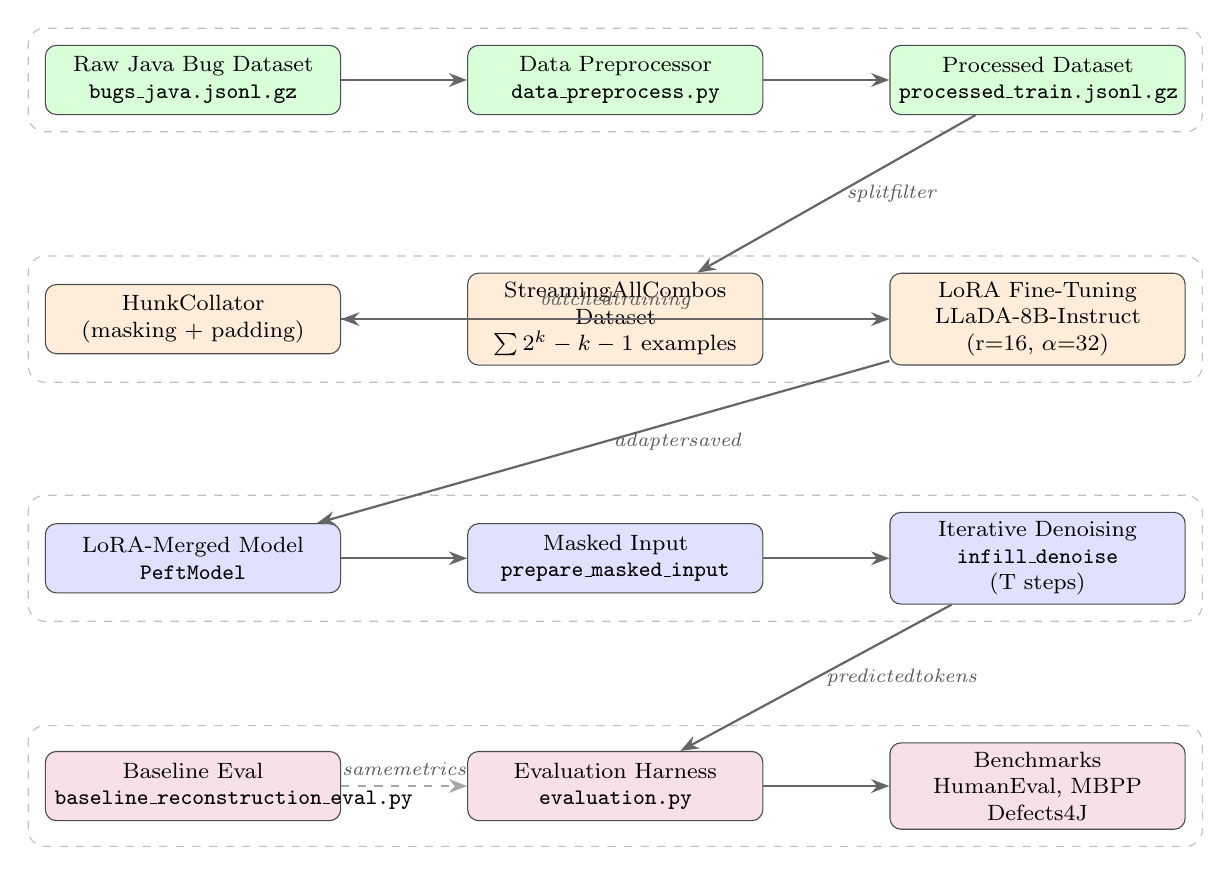
\begin{tikzpicture}[node distance=1.4cm and 1.8cm]

  %% ---- DATA STAGE ----
  \node[bigblock, fill=green!15] (raw) {Raw Java Bug Dataset\\\texttt{bugs\_java.jsonl.gz}};
  \node[bigblock, fill=green!15, right=1.6cm of raw] (preproc) {Data Preprocessor\\\texttt{data\_preprocess.py}};
  \node[bigblock, fill=green!15, right=1.6cm of preproc] (proc) {Processed Dataset\\\texttt{processed\_train.jsonl.gz}};

  \draw[arrow] (raw) -- (preproc);
  \draw[arrow] (preproc) -- (proc);

  %% ---- TRAINING STAGE ----
  \node[bigblock, fill=orange!15, below=2.0cm of preproc] (dataset) {StreamingAllCombos\\Dataset\\\(\sum 2^k - k - 1\) examples};
  \node[bigblock, fill=orange!15, left=1.6cm of dataset] (collator) {HunkCollator\\(masking + padding)};
  \node[bigblock, fill=orange!15, right=1.6cm of dataset] (lora) {LoRA Fine-Tuning\\LLaDA-8B-Instruct\\(r=16, \(\alpha\)=32)};

  \draw[arrow] (proc) -- node[right, label]{split\\filter} (dataset);
  \draw[arrow] (dataset) -- (collator);
  \draw[arrow] (collator) -- node[above, label]{batched\\training} (lora);

  %% ---- INFERENCE STAGE ----
  \node[bigblock, fill=blue!12, below=2.0cm of dataset] (maskedinput) {Masked Input\\\texttt{prepare\_masked\_input}};
  \node[bigblock, fill=blue!12, right=1.6cm of maskedinput] (denoise) {Iterative Denoising\\\texttt{infill\_denoise}\\(T steps)};
  \node[bigblock, fill=blue!12, left=1.6cm of maskedinput] (loramodel) {LoRA-Merged Model\\\texttt{PeftModel}};

  \draw[arrow] (lora) -- node[right, label]{adapter\\saved} (loramodel);
  \draw[arrow] (loramodel) -- (maskedinput);
  \draw[arrow] (maskedinput) -- (denoise);

  %% ---- EVALUATION STAGE ----
  \node[bigblock, fill=purple!12, below=2.0cm of maskedinput] (eval) {Evaluation Harness\\\texttt{evaluation.py}};
  \node[bigblock, fill=purple!12, right=1.6cm of eval] (benchmarks) {Benchmarks\\HumanEval, MBPP\\Defects4J};
  \node[bigblock, fill=purple!12, left=1.6cm of eval] (baselines) {Baseline Eval\\\texttt{baseline\_reconstruction\_eval.py}};

  \draw[arrow] (denoise) -- node[right, label]{predicted\\tokens} (eval);
  \draw[arrow] (eval) -- (benchmarks);
  \draw[dasharrow] (baselines) -- node[above, label]{same\\metrics} (eval);

  %% ---- GROUP LABELS ----
  \begin{scope}[on background layer]
    \node[groupbox, fit=(raw)(preproc)(proc), label=north:\textbf{Stage 1: Data Pipeline}] {};
    \node[groupbox, fit=(dataset)(collator)(lora), label=north:\textbf{Stage 2: Training}] {};
    \node[groupbox, fit=(maskedinput)(denoise)(loramodel), label=north:\textbf{Stage 3: Inference}] {};
    \node[groupbox, fit=(eval)(benchmarks)(baselines), label=north:\textbf{Stage 4: Evaluation}] {};
  \end{scope}

\end{tikzpicture}
\caption{High-level system architecture of MDLM Bug Fixer. Green = data pipeline; orange = training; blue = inference; purple = evaluation.}
\label{fig:arch}
\end{figure}

%% ============================================================
\section{Data Pipeline}
\label{sec:data}
%% ============================================================

\subsection{Raw Data Format}

The raw dataset \texttt{bugs\_java.jsonl.gz} contains records with the following fields: a unique record ID, the buggy Java source (\texttt{old}), and the fixed Java source (\texttt{new}). Each file pair may contain zero to many textual hunks.

\subsection{Hunk Identification}

We use Python's \texttt{difflib.SequenceMatcher} to compute the unified diffs between the \texttt{old} and \texttt{new} versions (Algorithm~\ref{alg:diff}). Non-equal opcodes are collected as hunks \((i_1, i_2, j_1, j_2)\) representing line ranges in the old and new files, respectively. Character-level spans in the \emph{fixed} file are computed from these hunk boundaries.

\begin{algorithm}[H]
\caption{Hunk Span Extraction}
\label{alg:diff}
\begin{algorithmic}[1]
\Require Buggy source $S_{\text{old}}$, fixed source $S_{\text{new}}$
\Ensure List of character spans $\{(s_i, e_i)\}$ in $S_{\text{new}}$
\State Split $S_{\text{old}}, S_{\text{new}}$ into line arrays
\State Compute opcodes via \texttt{SequenceMatcher}
\State $\mathcal{H} \gets \{(i_1,i_2,j_1,j_2) \mid \text{opcode} \neq \text{"equal"}\}$
\State Compute character offset array from $S_{\text{new}}$ lines
\For{each hunk $(i_1, i_2, j_1, j_2) \in \mathcal{H}$}
  \State $s \gets \text{offset}[j_1],\quad e \gets \text{offset}[j_2{-}1] + \text{len}(\text{line}[j_2{-}1])$
  \State Append $(s, e)$ to spans
\EndFor
\State Map spans to token-level spans via tokeniser offset mapping
\State Filter overlapping or out-of-range spans; cap to \texttt{HUNK\_CAP}$=5$
\end{algorithmic}
\end{algorithm}

\subsection{Tokenisation and Multi-Combo Expansion}

Each record is tokenised using the LLaDA-8B-Instruct tokeniser (max length 2048). Character spans are mapped to token spans using the tokeniser's offset mapping. Records with fewer than two valid hunk spans are discarded.

For a record with $k$ valid hunks, we generate all subsets of size $\geq 2$:
\[
  N_{\text{train}}(k) = \sum_{r=2}^{k} \binom{k}{r} = 2^k - k - 1
\]
This forces the model to learn to infer any subset of hunks given the remaining hunk context, building robustness to partial information. The processed dataset is written to \texttt{processed\_train.jsonl.gz} with fields: \texttt{record\_id}, \texttt{input\_ids} (fixed-file token IDs), \texttt{hunk\_token\_spans}, and \texttt{mask\_token\_id}.

\subsection{Train/Test Split}

A deterministic hash-based split assigns 10\% of records to the \texttt{test} split:
\[
  \text{split}(r) = \begin{cases} \text{test} & \text{if } \frac{\text{SHA-256}(\text{seed:}r)_{[0:8]}}{2^{32}} < 0.1 \\ \text{train} & \text{otherwise} \end{cases}
\]
This ensures reproducibility across preprocessing, training, and inference without materialising separate files.

%% ============================================================
\section{Model and Training}
\label{sec:model}
%% ============================================================

\subsection{Base Model: LLaDA-8B-Instruct}

LLaDA (Large Language Diffusion with mAsking) is an 8B-parameter masked diffusion language model trained to predict masked tokens given unmasked context, analogous to BERT but at generative scale. It uses a special \texttt{<|mdm\_mask|>} token (vocab ID 126336) as its noise state. During training, a subset of tokens is replaced with \texttt{<|mdm\_mask|>} and the model is supervised to reconstruct them via cross-entropy loss on the masked positions only.

\subsection{LoRA Fine-Tuning}

We apply LoRA~\cite{lora} to the attention and MLP projection layers:

\begin{center}
\begin{tabular}{ll}
\toprule
\textbf{Hyperparameter} & \textbf{Value}\\
\midrule
LoRA rank $r$ & 16\\
LoRA $\alpha$ & 32\\
LoRA dropout & 0.05\\
Target modules & \texttt{q\_proj, k\_proj, v\_proj, o\_proj,}\\
               & \texttt{up\_proj, down\_proj, gate\_proj}\\
Batch size (per device) & 1\\
Gradient accumulation & 4 steps (effective batch = 4)\\
Precision & BFloat16 (with float32 fallback)\\
Gradient checkpointing & enabled\\
\bottomrule
\end{tabular}
\end{center}

\subsection{Training Objective}

Given an input sequence with hunk tokens replaced by \texttt{<|mdm\_mask|>}, the model predicts the original tokens. The loss is masked cross-entropy applied exclusively to the hunk (masked) positions:
\[
  \mathcal{L} = -\frac{1}{|\mathcal{M}|} \sum_{i \in \mathcal{M}} \log P_\theta(x_i \mid \tilde{\mathbf{x}})
\]
where $\mathcal{M}$ is the set of masked token positions and $\tilde{\mathbf{x}}$ is the corrupted input. Non-hunk tokens contribute zero gradient via \texttt{labels}$= -100$.

%% ============================================================
\section{Inference: Iterative Denoising}
\label{sec:inference}
%% ============================================================

\subsection{Algorithm}

At inference, all hunk token positions of a test record are masked. The model then iteratively uncovers tokens in a scheduled fashion (Figure~\ref{fig:denoise}).

\begin{algorithm}[H]
\caption{Confidence-Ordered Iterative Denoising (\texttt{infill\_denoise})}
\label{alg:denoise}
\begin{algorithmic}[1]
\Require Masked input $\tilde{\mathbf{x}}$, mask positions $\mathcal{M}$, steps $T$, temperature $\tau$
\State $\mathbf{x} \gets \tilde{\mathbf{x}}$;\quad $\text{still\_masked} \gets \mathcal{M}$
\State Compute linear schedule: $[k_1, \ldots, k_T]$ summing to $|\mathcal{M}|$
\For{step $t = 1 \ldots T$}
  \State $\mathbf{L} \gets \text{model}(\mathbf{x})$\hfill\Comment{Forward pass}
  \If{$\tau = 0$} $\hat{\mathbf{x}} \gets \arg\max \mathbf{L}$\hfill\Comment{Greedy}
  \Else{} $\hat{\mathbf{x}} \gets$ Gumbel-max sample of $\mathbf{L}$ at temperature $\tau$
  \EndIf
  \State $\text{conf}_i \gets P_\theta(\hat{x}_i \mid \mathbf{x})$ for $i \in \text{still\_masked}$
  \State $\mathcal{T} \gets$ top-$k_t$ indices by $\text{conf}$\hfill\Comment{Most confident first}}
  \State $\mathbf{x}[\mathcal{T}] \gets \hat{\mathbf{x}}[\mathcal{T}]$;\quad $\text{still\_masked} \gets \text{still\_masked} \setminus \mathcal{T}$
  \State $\mathbf{x}[\text{still\_masked}] \gets \texttt{<|mdm\_mask|>}$\hfill\Comment{Re-mask remaining}
\EndFor
\State \Return $\mathbf{x}$
\end{algorithmic}
\end{algorithm}

\medskip
The schedule $[k_1, \ldots, k_T]$ is produced by a linear allocation:
\[
  k_t = \left\lfloor \frac{|\mathcal{M}|}{T} \right\rfloor + \mathbf{1}[t \leq |\mathcal{M}| \bmod T]
\]
Two re-masking strategies are supported:
\begin{itemize}[noitemsep]
  \item \textbf{low\_confidence}: at each step, only the $k_t$ most confident predictions are committed; the rest are re-masked for the next step.
  \item \textbf{random}: positions to unmask at each step are drawn uniformly at random from the remaining masked set.
\end{itemize}

\subsection{Denoising Process Diagram}

\begin{figure}[H]
\centering
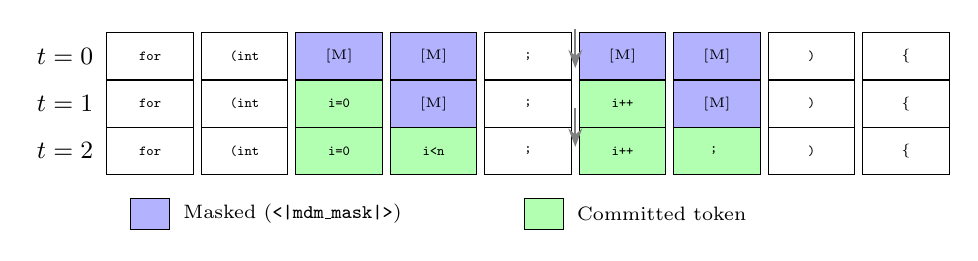
\begin{tikzpicture}[node distance=0.9cm and 1.4cm]

  \def\seqlen{9}
  \def\rowH{0.6}

  %% t=0 row
  \foreach \i/\col/\lbl in {
    0/white/\texttt{for},
    1/white/\texttt{(int},
    2/blue!30/[M],
    3/blue!30/[M],
    4/white/\texttt{;},
    5/blue!30/[M],
    6/blue!30/[M],
    7/white/\texttt{)},
    8/white/\texttt{\{}}
  {
    \node[draw, minimum width=1.1cm, minimum height=0.6cm, fill=\col, font=\tiny, align=center] at (\i*1.2, 2*\rowH) {\lbl};
  }
  \node[left, font=\small\bfseries] at (-0.6+0.0, 2*\rowH) {$t=0$};

  %% t=1 row (confident unmask of 2)
  \foreach \i/\col/\lbl in {
    0/white/\texttt{for},
    1/white/\texttt{(int},
    2/green!30/\texttt{i=0},
    3/blue!30/[M],
    4/white/\texttt{;},
    5/green!30/\texttt{i++},
    6/blue!30/[M],
    7/white/\texttt{)},
    8/white/\texttt{\{}}
  {
    \node[draw, minimum width=1.1cm, minimum height=0.6cm, fill=\col, font=\tiny, align=center] at (\i*1.2, 1*\rowH) {\lbl};
  }
  \node[left, font=\small\bfseries] at (-0.6+0.0, 1*\rowH) {$t=1$};

  %% t=2 row (fully resolved)
  \foreach \i/\col/\lbl in {
    0/white/\texttt{for},
    1/white/\texttt{(int},
    2/green!30/\texttt{i=0},
    3/green!30/\texttt{i<n},
    4/white/\texttt{;},
    5/green!30/\texttt{i++},
    6/green!30/\texttt{;}\ ,
    7/white/\texttt{)},
    8/white/\texttt{\{}}
  {
    \node[draw, minimum width=1.1cm, minimum height=0.6cm, fill=\col, font=\tiny, align=center] at (\i*1.2, 0*\rowH) {\lbl};
  }
  \node[left, font=\small\bfseries] at (-0.6+0.0, 0*\rowH) {$t=2$};

  %% Arrows
  \draw[arrow, gray] (5.4, 1.55) -- (5.4, 1.05);
  \draw[arrow, gray] (5.4, 0.55) -- (5.4, 0.05);

  %% Legend
  \node[draw, fill=blue!30, minimum width=0.5cm, minimum height=0.4cm] at (0, -0.8) {};
  \node[right, font=\scriptsize] at (0.3, -0.8) {Masked (\texttt{<|mdm\_mask|>})};
  \node[draw, fill=green!30, minimum width=0.5cm, minimum height=0.4cm] at (5, -0.8) {};
  \node[right, font=\scriptsize] at (5.3, -0.8) {Committed token};

\end{tikzpicture}
\caption{Schematic of the iterative denoising process. Blue cells are masked positions; green cells have been committed based on model confidence. Unmasked (white) tokens provide context throughout all steps.}
\label{fig:denoise}
\end{figure}

%% ============================================================
\section{Baselines}
\label{sec:baselines}
%% ============================================================

We evaluate two families of zero-shot baselines, all sharing the same \texttt{evaluation.py} metrics.

\subsection{Strategy A: FIM Chaining}

Fill-in-the-Middle models are applied hunk-by-hunk. After each hunk is filled, the working source is updated so that downstream hunks see already-repaired context—mirroring the progressive unmasking of MDLM inference.

\begin{center}
\begin{tabular}{lll}
\toprule
\textbf{Tag} & \textbf{Model} & \textbf{FIM Template} \\
\midrule
\texttt{deepseek-coder} & \texttt{deepseek-ai/deepseek-coder-6.7b-base} & \texttt{<|fim\_begin|>} ... \texttt{<|fim\_hole|>} ... \texttt{<|fim\_end|>} \\
\texttt{starcoder2}     & \texttt{bigcode/starcoder2-7b}              & \texttt{<fim\_prefix>} ... \texttt{<fim\_suffix>} ... \texttt{<fim\_middle>} \\
\texttt{codellama}      & \texttt{codellama/CodeLlama-7b-hf}          & \texttt{<PRE>} ... \texttt{<SUF>} ... \texttt{<MID>} \\
\bottomrule
\end{tabular}
\end{center}

\subsection{Strategy B: Instruction Zero-Shot}

A single prompt enumerates all masked regions and asks the model to return \texttt{PATCH\_i} blocks. No fine-tuning. This represents the minimal AR reference.

\begin{center}
\begin{tabular}{lll}
\toprule
\textbf{Tag} & \textbf{Model} & \textbf{Notes} \\
\midrule
\texttt{qwen} & \texttt{Qwen/Qwen2.5-Coder-7B-Instruct} & pass@\(k\) sampling supported \\
\texttt{deepseek-instruct} & \texttt{deepseek-ai/deepseek-coder-7b-instruct-v1.5} & pass@\(k\) sampling supported \\
\bottomrule
\end{tabular}
\end{center}

\subsection{Baseline Limitations}

\begin{itemize}[noitemsep]
  \item FIM models have no cross-hunk attention during a single forward pass; each hunk is repaired independently.
  \item Instruct models lack any fine-tuning on the structured multi-hunk format; they may produce incorrectly formatted \texttt{PATCH\_i} responses.
  \item All baselines are zero-shot; MDLM has the advantage of task-specific LoRA adaptation.
\end{itemize}

\subsection{Baseline Strategy Diagram}

\begin{figure}[H]
\centering
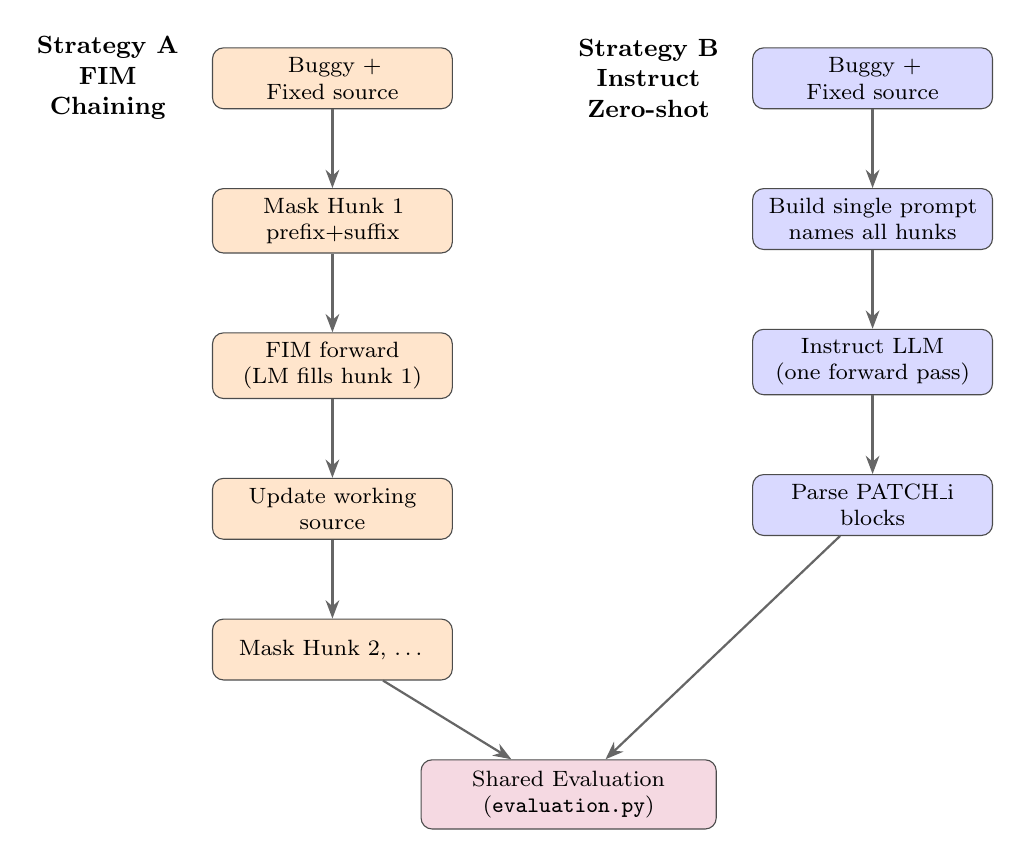
\begin{tikzpicture}[node distance=1.1cm and 2.0cm]

  %% FIM Path
  \node[wideblock, fill=orange!20] (bugsrc) {Buggy + Fixed source};
  \node[wideblock, fill=orange!20, below=1.0cm of bugsrc] (hunk1) {Mask Hunk 1\\\footnotesize prefix+suffix};
  \node[wideblock, fill=orange!20, below=1.0cm of hunk1] (fim1)  {FIM forward\\\footnotesize (LM fills hunk 1)};
  \node[wideblock, fill=orange!20, below=1.0cm of fim1]  (update){Update working\\\footnotesize source};
  \node[wideblock, fill=orange!20, below=1.0cm of update] (hunk2) {Mask Hunk 2, \ldots};

  \draw[arrow] (bugsrc) -- (hunk1);
  \draw[arrow] (hunk1) -- (fim1);
  \draw[arrow] (fim1) -- (update);
  \draw[arrow] (update) -- (hunk2);

  \node[left=0.3cm of bugsrc, font=\small\bfseries, align=center] {\textbf{Strategy A}\\FIM\\Chaining};

  %% Instruct Path
  \node[wideblock, fill=blue!15, right=3.8cm of bugsrc] (src2) {Buggy + Fixed source};
  \node[wideblock, fill=blue!15, below=1.0cm of src2] (prompt) {Build single prompt\\\footnotesize names all hunks};
  \node[wideblock, fill=blue!15, below=1.0cm of prompt] (llm)  {Instruct LLM\\\footnotesize (one forward pass)};
  \node[wideblock, fill=blue!15, below=1.0cm of llm]  (parse) {Parse PATCH\_i\\\footnotesize blocks};

  \draw[arrow] (src2) -- (prompt);
  \draw[arrow] (prompt) -- (llm);
  \draw[arrow] (llm) -- (parse);

  \node[left=0.3cm of src2, font=\small\bfseries, align=center] {\textbf{Strategy B}\\Instruct\\Zero-shot};

  %% Common eval node
  \node[bigblock, fill=purple!15, below=1.0cm of hunk2, xshift=3.0cm] (eval2) {Shared Evaluation\\(\texttt{evaluation.py})};
  \draw[arrow] (hunk2) -- (eval2);
  \draw[arrow] (parse) -- (eval2);

\end{tikzpicture}
\caption{Side-by-side comparison of the two baseline strategies. Both feed into the shared evaluation harness.}
\label{fig:baselines}
\end{figure}

%% ============================================================
\section{Evaluation Metrics}
\label{sec:metrics}
%% ============================================================

All metrics are implemented in \texttt{evaluation.py} and shared across MDLM and baselines.

\begin{center}
\renewcommand{\arraystretch}{1.25}
\begin{tabular}{p{4.5cm} p{8.5cm}}
\toprule
\textbf{Metric} & \textbf{Description} \\
\midrule
Token Exact Match Rate & Fraction of ground-truth token positions correctly predicted (variable-length safe). \\[2pt]
Per-Hunk Exact Match & For each hunk span $[s, e)$, checks if \emph{all} tokens in the span match. \\[2pt]
All-Hunks Correct & Boolean: 1 iff every hunk in the record is exactly correct. \\[2pt]
Patch String EM & String-level exact match after Unicode NFC normalisation. \\[2pt]
Normalised Edit Distance & Levenshtein distance normalised by $\max(|\hat{y}|, |y|)$; range $[0,1]$. \\[2pt]
Patch BLEU-4 & Sentence BLEU-4 on whitespace-tokenised patch text; no external deps. \\[2pt]
CodeBLEU & Weighted combination of BLEU + AST match + data-flow match~\cite{codebleu}. \\[2pt]
Masked Cross-Entropy & Cross-entropy loss on masked positions only (MDLM-specific). \\[2pt]
Top-$k$ Accuracy & Whether ground-truth token appears in top-$k$ logit positions. \\[2pt]
pass@$k$ & Unbiased estimator from~\cite{humaneval}: $\Pr[\geq 1$ correct in $k$ draws$]$. \\
\bottomrule
\end{tabular}
\end{center}

\subsection{Benchmarks}

\paragraph{Internal reconstruction benchmark.} Evaluates on the held-out \texttt{test} split (10\% of records) from \texttt{processed\_train.jsonl.gz}. Records with $k \geq 2$ valid hunks, evaluated on the full hunk subset.

\paragraph{Defects4J benchmark.} An oracle-localised evaluation on real Java bugs. The pipeline:
\begin{enumerate}[noitemsep]
  \item Checks out the buggy version with \texttt{defects4j checkout}.
  \item Diffs buggy vs.\ fixed modified Java files to identify hunks.
  \item Masks those hunks and runs iterative denoising.
  \item Optionally compiles and runs the test suite in the checkout directory.
\end{enumerate}
Projects evaluated: \texttt{Lang}, \texttt{Math} (configurable).

\paragraph{EvalPlus benchmarks.} HumanEval+ and MBPP+ from the EvalPlus framework, adapted for LLaDA's append-and-denoise generation mode.

%% ============================================================
\section{Experimental Setup}
\label{sec:setup}
%% ============================================================

\begin{center}
\begin{tabular}{ll}
\toprule
\textbf{Setting} & \textbf{Value} \\
\midrule
Base model & \texttt{GSAI-ML/LLaDA-8B-Instruct} \\
Tokeniser & LLaDA-8B-Instruct fast tokeniser \\
Max sequence length & 2048 (preprocessing) / model config (training) \\
Test fraction & 10\% (hash-based, seed=42) \\
Training records (full run) & 1000 base records \\
Evaluation records & 200 records per system \\
Denoising steps $T$ & 64 (default) \\
Temperature $\tau$ & 0.0 (greedy) \\
Re-masking strategy & \texttt{low\_confidence} \\
Hunk cap per file & 5 \\
Hardware & 1$\times$ NVIDIA A100 (40 GB), 32 GB RAM \\
Deployment & Kubernetes Jobs (k8s/ manifests) \\
\bottomrule
\end{tabular}
\end{center}

%% ============================================================
\section{Results}
\label{sec:results}
%% ============================================================

\subsection{Internal Reconstruction Benchmark}

Table~\ref{tab:reconstruction} reports model performance on the held-out test split.

\begin{table}[H]
\centering
\caption{Reconstruction benchmark results on the held-out test split (\(N = 200\) records). Best result per column is \textbf{bolded}. \textit{(Populate with experimental numbers.)}}
\label{tab:reconstruction}
\renewcommand{\arraystretch}{1.2}
\begin{tabular}{lccccccc}
\toprule
\textbf{System} & \textbf{All-Hunks} & \textbf{Hunk EM} & \textbf{Token EM} & \textbf{Patch EM} & \textbf{NED}$\downarrow$ & \textbf{BLEU-4} & \textbf{CodeBLEU} \\
 & \textbf{Correct (\%)} & \textbf{(\%)} & \textbf{Rate (\%)} & \textbf{(\%)} & & & \\
\midrule
LLaDA-8B (no LoRA)        & -- & -- & -- & -- & -- & -- & -- \\
\textbf{LLaDA-8B + LoRA}  & -- & -- & -- & -- & -- & -- & -- \\
\midrule
DeepSeek-Coder FIM        & -- & -- & -- & -- & -- & -- & -- \\
StarCoder2 FIM            & -- & -- & -- & -- & -- & -- & -- \\
CodeLlama FIM             & -- & -- & -- & -- & -- & -- & -- \\
\midrule
Qwen2.5-Coder Instruct    & -- & -- & -- & -- & -- & -- & -- \\
DeepSeek-Instruct         & -- & -- & -- & -- & -- & -- & -- \\
\bottomrule
\end{tabular}
\end{table}

\subsection{Defects4J Java SWE Benchmark}

Table~\ref{tab:defects4j} reports bug-level performance on the Defects4J benchmark.

\begin{table}[H]
\centering
\caption{Defects4J oracle-localised benchmark. File-level and bug-level results. Compile and test-suite pass rates require Defects4J environment. \textit{(Populate with experimental numbers.)}}
\label{tab:defects4j}
\renewcommand{\arraystretch}{1.2}
\begin{tabular}{lcccccc}
\toprule
\textbf{Project} & \textbf{Bugs} & \textbf{Files Correct} & \textbf{Bugs Fully} & \textbf{Compile} & \textbf{Tests} & \textbf{CodeBLEU} \\
                 & \textbf{Tested} & \textbf{(\%)} & \textbf{Repaired (\%)} & \textbf{Pass (\%)} & \textbf{Pass (\%)} & \\
\midrule
Lang  & -- & -- & -- & -- & -- & -- \\
Math  & -- & -- & -- & -- & -- & -- \\
\midrule
\textbf{Total} & -- & -- & -- & -- & -- & -- \\
\bottomrule
\end{tabular}
\end{table}

\subsection{EvalPlus: HumanEval and MBPP}

Table~\ref{tab:evalplus} compares MDLM on standard code generation benchmarks.

\begin{table}[H]
\centering
\caption{EvalPlus results: pass@1 (greedy) and pass@10 (\(\tau=0.6\), 10 samples). \textit{(Populate with experimental numbers.)}}
\label{tab:evalplus}
\renewcommand{\arraystretch}{1.2}
\begin{tabular}{lcccc}
\toprule
\textbf{Model} & \multicolumn{2}{c}{\textbf{HumanEval+}} & \multicolumn{2}{c}{\textbf{MBPP+}} \\
\cmidrule(lr){2-3}\cmidrule(lr){4-5}
 & pass@1 & pass@10 & pass@1 & pass@10 \\
\midrule
LLaDA-8B (no LoRA)       & -- & -- & -- & -- \\
LLaDA-8B + LoRA          & -- & -- & -- & -- \\
\midrule
DeepSeek-Coder-6.7B      & -- & -- & -- & -- \\
Qwen2.5-Coder-7B-Instruct& -- & -- & -- & -- \\
\bottomrule
\end{tabular}
\end{table}

\subsection{Effect of Denoising Steps}
\label{sec:abl_steps}

We study the effect of the number of denoising steps \(T\). Too few steps limit
refinement, while too many steps increase latency with potentially diminishing
returns. All runs use the LoRA-adapted model with greedy decoding
(\(\tau=0\)) and \texttt{low\_confidence} re-masking.

\begin{table}[H]
\centering
\caption{Effect of denoising steps $T$ on reconstruction quality
(LLaDA-8B + LoRA, greedy, \texttt{low\_confidence} remasking,
$N=200$ test records).
Tables auto-generated by \texttt{run\_ablations.py}.
\textit{Populate with final numbers.}}
\label{tab:ablation_steps}
\renewcommand{\arraystretch}{1.15}
\begin{tabular}{lccccc}
\toprule
\textbf{Steps $T$} & \textbf{All-Hunks (\%)} & \textbf{Token EM (\%)} & \textbf{BLEU-4} & \textbf{CodeBLEU} & \textbf{Latency (s/sample)} \\
\midrule
1   & -- & -- & -- & -- & -- \\
16  & -- & -- & -- & -- & -- \\
32  & -- & -- & -- & -- & -- \\
64  & -- & -- & -- & -- & -- \\
128 & -- & -- & -- & -- & -- \\
\bottomrule
\end{tabular}
\end{table}

\subsection{Effect of Re-Masking Strategy}
\label{sec:abl_remask}

We compare \texttt{low\_confidence} re-masking—which commits the \(k_t\) most
confident tokens at each step—against \texttt{random} re-masking, which
commits a uniformly random subset. Both are evaluated at fixed \(T=64\) with
the LoRA model.

\begin{table}[H]
\centering
\caption{Re-masking strategy comparison with fixed denoising steps ($T=64$,
LLaDA-8B + LoRA, greedy, $N=200$ test records).
\textit{Populate with final numbers.}}
\label{tab:ablation_remask}
\renewcommand{\arraystretch}{1.15}
\begin{tabular}{lccccc}
\toprule
\textbf{Re-masking} & \textbf{All-Hunks (\%)} & \textbf{Hunk EM (\%)} & \textbf{Token EM (\%)} & \textbf{BLEU-4} & \textbf{CodeBLEU} \\
\midrule
\texttt{low\_confidence} & -- & -- & -- & -- & -- \\
\texttt{random}          & -- & -- & -- & -- & -- \\
\bottomrule
\end{tabular}
\end{table}

\subsection{Effect of Fine-Tuning}
\label{sec:abl_finetune}

A core ablation compares the base LLaDA-8B-Instruct model against the
LoRA-adapted repair model, both evaluated with \(T=64\) and
\texttt{low\_confidence} re-masking. This isolates the contribution of
task-specific fine-tuning from the general masked diffusion prior inherited
from pre-training. We expect the base model to show non-trivial performance
(the MDLM prior already handles infilling), with the LoRA adapter providing
the remaining accuracy gains by specialising to Java bug patterns and the
multi-hunk training format.

\begin{table}[H]
\centering
\caption{Effect of LoRA fine-tuning versus base LLaDA-8B-Instruct
($T=64$, greedy, \texttt{low\_confidence} remasking, $N=200$ test records).
\textit{Populate with final numbers.}}
\label{tab:ablation_finetune}
\renewcommand{\arraystretch}{1.15}
\begin{tabular}{lccccccc}
\toprule
\textbf{Model} & \textbf{All-Hunks} & \textbf{Hunk EM} & \textbf{Token EM}
  & \textbf{Patch EM} & \textbf{BLEU-4} & \textbf{CodeBLEU} & \textbf{CE}$\downarrow$ \\
 & \textbf{(\%)} & \textbf{(\%)} & \textbf{(\%)} & \textbf{(\%)} & & & \\
\midrule
LLaDA-8B (base)  & -- & -- & -- & -- & -- & -- & -- \\
LLaDA-8B + LoRA  & -- & -- & -- & -- & -- & -- & -- \\
\bottomrule
\end{tabular}
\end{table}

\paragraph{Running all ablations.}
All three ablation axes are orchestrated by \texttt{run\_ablations.py}:

\begin{lstlisting}[style=python, caption={Running the full ablation suite locally.}]
# Full run (200 records, CodeBLEU enabled)
python run_ablations.py --max-records 200 --codebleu

# Quick sanity check (5 records)
python run_ablations.py --dry-run

# Run only one axis
python run_ablations.py --ablation steps --max-records 200
\end{lstlisting}

The script saves \texttt{runs/ablations/ablation\_all.json} (raw metrics) and
\texttt{runs/ablations/ablation\_tables.tex} (LaTeX tables ready to paste into
this report). It models are loaded once per checkpoint: the LoRA model is
reused across Ablations~\ref{sec:abl_steps}, \ref{sec:abl_remask}, and the
LoRA arm of~\ref{sec:abl_finetune}; the base model is loaded only for the
final arm, and freed immediately afterwards to conserve GPU memory.

%% ============================================================
\section{Deployment and Infrastructure}
\label{sec:infra}
%% ============================================================

All training and evaluation jobs are deployed as Kubernetes batch jobs. Table~\ref{tab:k8s} lists the available manifests.

\begin{table}[H]
\centering
\caption{Kubernetes job manifests in \texttt{k8s/}.}
\label{tab:k8s}
\renewcommand{\arraystretch}{1.2}
\begin{tabular}{ll}
\toprule
\textbf{Manifest} & \textbf{Purpose} \\
\midrule
\texttt{train-job.yaml}          & Full LoRA fine-tuning job (A100, BFloat16) \\
\texttt{benchmark-job.yaml}      & MDLM reconstruction benchmark \\
\texttt{benchmark-base-job.yaml} & Base LLaDA (no LoRA) reconstruction benchmark \\
\texttt{benchmark-bcb-job.yaml}  & BigCodeBench evaluation \\
\texttt{swe\_benchmark.yaml}     & Defects4J Java SWE benchmark \\
\texttt{ablation-job.yaml}       & All three ablation axes (\texttt{run\_ablations.py}) \\
\texttt{pvc-outputs.yaml}        & Persistent volume for output artefacts \\
\texttt{jupyter-notebook.yaml}   & Interactive analysis environment \\
\bottomrule
\end{tabular}
\end{table}

Resource requirements per job: 1$\times$ NVIDIA A100 (80\,GB SXM4) GPU.
Training and ablation jobs request 48\,GiB RAM / 4 CPU cores; benchmark jobs
request 32\,GiB RAM / 2 CPU cores.

The ablation job \texttt{k8s/ablation-job.yaml} mirrors the structure of
\texttt{swe\_benchmark.yaml}: it clones the repository from the
\texttt{GIT\_BRANCH} env variable, resolves the LoRA adapter and processed
dataset from the PVC, runs \texttt{run\_ablations.py}, and prints the
full LaTeX tables to stdout at the end so they can be collected with
\texttt{kubectl logs}.

%% ============================================================
\section{Discussion}
\label{sec:discussion}
%% ============================================================

\paragraph{Advantages of MDLM for multi-hunk repair.}
Unlike FIM chaining, MDLM attends to all masked regions simultaneously at each denoising step. This enables the model to capture cross-hunk dependencies (e.g., a variable renamed in hunk 1 must appear in hunk 2), which is structurally impossible within a single FIM forward pass.

\paragraph{Training data amplification.}
The $2^k - k - 1$ combo expansion turns a single $k$-hunk record into up to 57 training examples ($k=6$), dramatically amplifying the effective training set size while teaching the model to infer hunk content from partial context.

\paragraph{Known limitations.}
\begin{itemize}[noitemsep]
  \item The model requires oracle hunk localisation at inference time; it is not yet a repository-level issue-solving agent.
  \item Sequence length is capped at 2048 tokens, limiting applicability to larger Java files.
  \item Evaluation is currently restricted to exact-match and surface-level metrics; semantic correctness requires test-suite execution.
\end{itemize}

\paragraph{Benchmark discrepancy note.}
As recorded in project notes, there is a current mismatch: \texttt{inference.py} evaluates on \texttt{split=test}, while \texttt{baseline\_reconstruction\_eval.py} loads the first $N$ records from \texttt{processed\_train.jsonl.gz} without split filtering. Results comparisons should account for this until the split filtering is unified.

%% ============================================================
\section{Conclusion}
\label{sec:conclusion}
%% ============================================================

We presented MDLM Bug Fixer, a system for multi-hunk Java bug repair using LLaDA-8B-Instruct fine-tuned with LoRA. The key insight is that masked diffusion provides a natural framework for simultaneous multi-region code infilling, with iterative confidence-based denoising enabling progressive refinement of all hunks in parallel. Our training data pipeline expands multi-hunk records into all valid subset combinations, ensuring robust coverage of partial-hunk inference scenarios.

Future work includes: (1) removing the oracle localisation requirement using a bug-detection head; (2) extending context to full repository files via efficient attention; (3) applying MDLM to Python SWE-bench for cross-language validation; and (4) integrating test-suite feedback into the denoising loop as a reward signal.

%% ============================================================
\appendix
\section{Prompt Templates for Diagram Generation}
\label{sec:prompts}
%% ============================================================

The following text boxes contain detailed prompts that can be fed to a diagram generation tool (e.g., ChatGPT + DALL-E, Mermaid, or draw.io) to produce publication-quality figures. The TikZ diagrams in the body of this report already provide functional versions; these prompts are for higher-fidelity alternatives.

\medskip

%% ---- PROMPT 1 ----
\begin{mdframed}[linecolor=blue!60, linewidth=1.2pt, roundcorner=6pt, backgroundcolor=blue!4]
\textbf{Prompt 1 — System Architecture Diagram}

\medskip
Draw a detailed software architecture diagram for a system called \textbf{MDLM Bug Fixer}. Use a vertical top-to-bottom layout with four clearly labeled horizontal lanes (or swimlanes):

\begin{enumerate}
  \item \textbf{Stage 1 — Data Pipeline (green):} Show a raw gzip JSONL file (\texttt{bugs\_java.jsonl.gz}) feeding into a preprocessing module that (a) computes unified diffs with \texttt{difflib.SequenceMatcher}, (b) tokenises with the LLaDA tokeniser, (c) maps character spans to token spans, and (d) expands each $k$-hunk record into $2^k - k - 1$ training examples. Output is \texttt{processed\_train.jsonl.gz}. Include a hash-based train/test splitter (10\% test).
  
  \item \textbf{Stage 2 — Training (orange):} A custom \texttt{StreamingAllCombosDataset} feeds a \texttt{HunkCollator} (which masks chosen hunk positions with \texttt{<|mdm\_mask|>} and sets non-hunk labels to $-100$). The collated batches train \textbf{LLaDA-8B-Instruct} with LoRA ($r=16$, $\alpha=32$, targeting Q/K/V/O/MLP projections) using the HuggingFace \texttt{Trainer}. The LoRA adapter is saved to \texttt{runs/llada\_lora/lora\_adapter/}.
  
  \item \textbf{Stage 3 — Inference (blue):} A test record is loaded; its hunk positions are masked. A \texttt{PeftModel} (base LLaDA + LoRA adapter) performs iterative denoising: at each of $T=64$ steps, it runs a full forward pass, scores confidence on masked positions, commits the top-$k_t$ most confident tokens (or random if in random-remasking mode), and re-masks the rest.
  
  \item \textbf{Stage 4 — Evaluation (purple):} Three parallel evaluation paths: (a) internal reconstruction test split, (b) Defects4J Java SWE benchmark (checkout $\to$ diff $\to$ mask $\to$ denoise $\to$ compile $\to$ test), (c) EvalPlus (HumanEval+, MBPP+). A shared \texttt{evaluation.py} provides all metrics. Baselines (FIM chaining and instruct zero-shot) share the same evaluation harness.
\end{enumerate}

Use color-coded rounded rectangles for components and labeled arrows for data flow. Add a legend for colors. Make it suitable for an academic paper.
\end{mdframed}

\bigskip

%% ---- PROMPT 2 ----
\begin{mdframed}[linecolor=green!60!black, linewidth=1.2pt, roundcorner=6pt, backgroundcolor=green!4]
\textbf{Prompt 2 — Iterative Denoising Inference Diagram}

\medskip
Draw an animated-style step diagram showing the iterative denoising process of a Masked Diffusion Language Model (MDLM) applied to multi-hunk code repair. The diagram should show a \textbf{sequence of token rows} (left to right representing token positions in a Java code snippet), evolving over \textbf{denoising steps $t = 0, 1, \ldots, T$} (top to bottom).

Key visual elements:
\begin{itemize}
  \item Each row represents the state of the full token sequence at step $t$.
  \item Tokens belonging to the \textbf{unmasked context} (non-hunk code) are shown in \textbf{white/light gray} — they never change.
  \item Tokens in the \textbf{masked hunk regions} start as blue boxes labeled \texttt{[MASK]} at $t=0$.
  \item At each step, the model runs a forward pass over the whole sequence and computes a \textbf{confidence score} for each masked position.
  \item The top-$k_t$ most confident tokens are \textbf{committed} (shown in green with the actual token text, e.g., \texttt{i = 0}, \texttt{i < n}).
  \item Remaining masked positions are \textbf{re-masked} (blue boxes).
  \item The schedule $k_t$ is shown in a side column: e.g., commit 2 tokens at $t=1$, 2 more at $t=2$, etc.
  \item Show two separate hunk regions (Hunk A on the left, Hunk B on the right) evolving simultaneously, demonstrating cross-hunk parallelism.
  \item Add a confidence bar chart below each step showing the confidence scores for masked positions.
  \item At the final step $T$, all positions are committed and both hunks show correct Java code.
\end{itemize}

Style: clean, academic, suitable for a conference paper. Use blue for masked, green for committed, gray for context. Add step labels on the left.
\end{mdframed}

\bigskip

%% ---- PROMPT 3 ----
\begin{mdframed}[linecolor=orange!70!black, linewidth=1.2pt, roundcorner=6pt, backgroundcolor=orange!4]
\textbf{Prompt 3 — Data Pipeline and Multi-Combo Expansion Diagram}

\medskip
Draw a data pipeline diagram illustrating how a raw Java bug record is transformed into multiple training examples for MDLM fine-tuning.

The diagram should show the following steps from left to right (or top to bottom):

\begin{enumerate}
  \item \textbf{Input}: A side-by-side display of the \emph{buggy} Java method and the \emph{fixed} Java method, with 3 highlighted ``changed regions'' (Hunk 1, Hunk 2, Hunk 3).
  
  \item \textbf{Diff Computation}: An arrow pointing to a diff output showing the 3 hunks identified by \texttt{difflib}. Label: ``$k = 3$ hunks''.
  
  \item \textbf{Tokenisation}: The fixed Java method is tokenised. Show the token sequence as a horizontal array of boxes. The 3 hunk regions are highlighted in different colors. A bracket shows ``token span $[s_1, e_1)$'' etc.
  
  \item \textbf{Combo Expansion}: Show the formula $2^3 - 3 - 1 = 4$ training examples. Draw 4 copies of the token sequence, each with a different subset of 2 or more hunks masked:
    \begin{itemize}
      \item Example 1: Mask hunks \{1, 2\}
      \item Example 2: Mask hunks \{1, 3\}
      \item Example 3: Mask hunks \{2, 3\}
      \item Example 4: Mask hunks \{1, 2, 3\}
    \end{itemize}
    In each copy, masked hunk positions are shown as blue boxes (\texttt{[MASK]}), and non-masked hunk positions show their actual tokens.
  
  \item \textbf{Training Signal}: Show that the loss is computed only on the masked (blue) positions (red arrows pointing to loss boxes below each masked position). Non-masked tokens have $\text{label} = -100$.
\end{enumerate}

Use a clean academic style. Color code: green = known/context, blue = masked/target, red = loss signal.
\end{mdframed}

%% ============================================================
\begin{thebibliography}{99}

\bibitem{llada2024}
Nie, S., et al. (2025).
\textit{LLaDA: Large Language Diffusion with mAsking}.
arXiv preprint arXiv:2502.09992.

\bibitem{lora}
Hu, E. J., et al. (2022).
\textit{LoRA: Low-Rank Adaptation of Large Language Models}.
ICLR 2022.

\bibitem{codellama}
Rozière, B., et al. (2023).
\textit{Code Llama: Open Foundation Models for Code}.
arXiv:2308.12950.

\bibitem{starcoder2}
Lozhkov, A., et al. (2024).
\textit{StarCoder 2 and The Stack v2: The Next Generation}.
arXiv:2402.19173.

\bibitem{deepseek}
Guo, D., et al. (2024).
\textit{DeepSeek-Coder: When the Large Language Model Meets Programming}.
arXiv:2401.14196.

\bibitem{austin2021structured}
Austin, J., et al. (2021).
\textit{Structured Denoising Diffusion Models in Discrete State-Spaces}.
NeurIPS 2021.

\bibitem{sahoo2024mdlm}
Sahoo, S., et al. (2024).
\textit{Simple and Effective Masked Diffusion Language Models}.
arXiv:2406.07524.

\bibitem{bert}
Devlin, J., et al. (2019).
\textit{BERT: Pre-training of Deep Bidirectional Transformers for Language Understanding}.
NAACL 2019.

\bibitem{defects4j}
Just, R., et al. (2014).
\textit{Defects4J: A Database of Existing Faults to Enable Controlled Testing Studies for Java Programs}.
ISSTA 2014.

\bibitem{swebench}
Jimenez, C. E., et al. (2024).
\textit{SWE-bench: Can Language Models Resolve Real-World GitHub Issues?}
ICLR 2024.

\bibitem{humaneval}
Chen, M., et al. (2021).
\textit{Evaluating Large Language Models Trained on Code}.
arXiv:2107.03374.

\bibitem{codebleu}
Ren, S., et al. (2020).
\textit{CodeBLEU: a Method for Automatic Evaluation of Code Synthesis}.
arXiv:2009.10297.

\bibitem{genprog}
Le Goues, C., et al. (2012).
\textit{GenProg: A Generic Method for Automatic Software Repair}.
IEEE Trans. Software Eng.

\bibitem{drrepair}
Yasunaga, M., \& Liang, P. (2020).
\textit{Graph-based, Self-Supervised Program Repair from Diagnostic Feedback}.
ICML 2020.

\bibitem{chatrepair}
Xia, C. S., \& Zhang, L. (2023).
\textit{Keep the Conversation Going: Fixing 162 out of 337 Bugs for \$0.42 each using ChatGPT}.
arXiv:2304.00385.

\end{thebibliography}

\end{document}
